\documentclass{article}
% \documentclass[11pt,letterpaper]{article}

% if you need to pass options to natbib, use, e.g.:
%     \PassOptionsToPackage{numbers, compress}{natbib}
% before loading neurips_2020

% ready for submission
% \usepackage{neurips_2020}

% to compile a preprint version, e.g., for submission to arXiv, add add the
% [preprint] option:
%     \usepackage[preprint]{neurips_2020}

% to compile a camera-ready version, add the [final] option, e.g.:
%     \usepackage[final]{neurips_2020}

% to avoid loading the natbib package, add option nonatbib:
\usepackage{amsmath,amssymb,latexsym,amsthm,cleveref}
\usepackage{fullpage}
\usepackage{geometry}
\usepackage{textcomp}
\usepackage{xcolor}
\usepackage{varioref}
\usepackage{bm}
\usepackage[ruled]{algorithm2e}
\geometry{margin=1in}

\usepackage[preprint]{neurips_2020}
\usepackage[nonatbib]{neurips_2020}

\usepackage[utf8]{inputenc} % allow utf-8 input
\usepackage[T1]{fontenc}    % use 8-bit T1 fonts
\usepackage{hyperref}       % hyperlinks
\usepackage{url}            % simple URL typesetting
\usepackage{booktabs}       % professional-quality tables
\usepackage{amsfonts}       % blackboard math symbols
\usepackage{nicefrac}       % compact symbols for 1/2, etc.
\usepackage{microtype}      % microtypography

\usepackage{graphicx}

\graphicspath{ {./images/} }

\title{Program Synthesis with Reinforcement Learning (RL) of Structured Edits}

% The \author macro works with any number of authors. There are two commands
% used to separate the names and addresses of multiple authors: \And and \AND.
%
% Using \And between authors leaves it to LaTeX to determine where to break the
% lines. Using \AND forces a line break at that point. So, if LaTeX puts 3 of 4
% authors names on the first line, and the last on the second line, try using
% \AND instead of \And before the third author name.
\author{
}

\begin{document}

\maketitle

\section{Research Objectives}
\begin{itemize}
    \item \textbf{Determine whether RL methods can be used to improve the performance of coding assistants.} Once an agent has been trained to map code states to a policy over actions, those actions can be used to suggest potential code edits to a human user working on the code.
    \item \textbf{Determine whether functional (or expression-based) programming languages are more tractable for RL code synthesis.} While this project will work exclusively with a functional programming language (namely OCaml), we are interested in the comparison between our results and existing results on imperative languages, namely those produced in \href{https://arxiv.org/abs/1711.00740}{LEARNING TO REPRESENT PROGRAMS WITH GRAPHS}.
    \item \textbf{Determine the impact of type information on RL performance.} We plan to run comparisons of results with and without type information included in the information provided to the agent. Without this information provided, the agent must learn to infer type-information in most cases, so we would expect the inclusion of type-information to benefit performance.
    \item \textbf{Explore methods for improving selection of variables in the synthesis of code.} In the section \hyperref[sec:parameterization]{Parameterization of action distribution}, we describe a novel method for selecting actions that allows the agent to be sensitive to the semantics of variables. We hope to demonstrate that this method improves performance over a naive baseline (either a-priori fixed variable names or De Bruijn indices).

\end{itemize}

\section{Environment}
\hspace{16}To represent program edit actions we are taking inspiration from work in programming language theory, in specific the Hazel semantic editor and the Hazelnut calculus on which it is based. This describes a formal semantics for structure editing, which distinguishes itself from text editing in that all operations necessarily preserve syntactic structure. This has two benefits in our context. First, it prevents pointless edits which lead to unparsable program states. Second, it ensures that, since the code is always well-formed, we can always use static analysis, in particular but not limited to type checking, to determine which actions are applicable given the state of the code. To this effect, we augment the syntactic forms of the subset of Ocaml we’re targeting with empty holes, placeholder forms which allow us to represent program sketches (incomplete programs) in a way that still permits semantic analysis.

\hspace{16}Following Hazel, we internalize the position of the cursor (editing focus) within the code itself by means of a zippered AST. The mechanics of this structure precisely model possible cursor movements, ensuring both that the cursor position is always valid and that the cursor always indicates a semantically-meaningful portion of the syntax tree. For the typed portion of our investigations, we will employ the Hazelnut bidirectional gradually type system, both to determine the expected and current type at the cursor, and to augment the syntax tree with type ascriptions.

\hspace{16}More broadly, we are interested in a framing where the task of the agent is not merely to modify a program as-such, but instead to perform actions within a ‘virtual integrated development environment’ created for the agent. This semantic interface will use derived semantic information about current and past program states to dynamically shape the action space presented to the agent, both for the sake of ‘keeping it on the rails’ and contextualizing the syntax with additional semantic annotations.

\hspace{16}Longer-term, our hope is that such a virtual development environment could be extended to support more sophisticated forms of program synthesis, ensuring that the agent is always acting within a space which has been maximally enriched by the derivable static and dynamic properties of the current program sketch.

\hspace{16}(we also might want to add a section detailing the exact subset of ocaml we’re supporting; this might be a bit in-flux though)

\subsection{Summary}
\hspace{16}The environment is composed of a dictionary observation space, including information about the assignment, the code to solve the assignment, the cursor, a list of valid actions at the cursor position, and the variables that are in scope at the cursor position. These information are obtained and modified using OCaml, where an AST is constructed and modified. The code is represented via recursive sum types in OCaml, which is transformed into arrays of integers back to Python for the agent to train on. Any other additional information are arrays based on the indexing of the arrays passed back to Python. 

\hspace{}The source code of a .ml file is encoded using recursive sum types in OCaml and arrays of integers in Python. In OCaml, each expression is encoded as a product of its children, and an expression is encoded as a sum of all types of expressions. In Python, this AST is translated into a graph structure using two arrays:
\begin{enumerate}
    \item Each node in OCaml is translated into a unique integer, and all these nodes are listed in this nodes array in Python. If the tree has size $n$, then this array would be size $n$. 
    \item Each edge is encoded using the index of the nodes adjacent to the edge. Moreover, a third element indicating the type of the edge (i.e. first child, second child, etc.) is added to the edge representation. Additionally, we added edges that connect variables and their binding site so that the GNN may more easily interpret what the variable means.
\end{enumerate}

\subsection{Observation Space}
\subsubsection{Assignment index}
\hspace{16}At the start of every timestep, an assignment index is randomly chosen from a uniform distribution. For this assignment, a random student’s starter code is randomly chosen for the system to start training from. Unit tests for this assignment are also loaded to evaluate the performance of the system on this assignment and starter code. Since the index of the starter code chosen should not affect the training, and all other required information are included in other parts of the observation space, the starter code index will not be part of the observation space.

\subsubsection{Graph representation of AST}
\hspace{16}The AST is represented differently in OCaml and Python to exploit the advantages of each language. In OCaml, the AST is represented by a recursive sum type to better exploit the pattern matching functionality of OCaml. In Python, the recursive sum type representation needs to be converted into two arrays, one to represent the type of each node and one to represent the edges. To implement how the agent modifies the AST, we also added a cursor via a zippered AST. 

\hspace{16}Each type of expression (e.g. addition, if expression, let expression, etc.) is represented as a node in the tree, and its subexpressions are represented as its children. The leaf nodes are integers, booleans, and variables. In Python, this tree is represented by two arrays:
\begin{itemize}
    \item Each type of a node in OCaml is translated into a unique integer, and all these nodes are listed in this nodes array in Python. If the tree has size $n$, then this array would be size $n$. 
    \item Each edge is encoded using the index of the nodes adjacent to the edge. Moreover, a third element indicating the type of the edge (i.e. first child, second child, etc.) is added to the edge representation. Additionally, we added edges that connect variables and their binding site so that the GNN may more easily interpret what the variable means.
\end{itemize}

\hspace{16}In addition to the basic expressions, we also plan to add type information to the AST. For now, we only included type annotations for functions. These type annotations may serve as restrictions for which actions that the agent can type. In the future, we plan to append the type of each node as part of the observations space. 

\subsubsection{Type Inference}
\hspace{16}Our system includes type information for the agent to decide which actions may be performed. The type information are inferred via mostly bidirectional typing with a few modifications to further restrict the agent from doing type-incorrect actions. The modifications to bidirectional typing are listed below:
\begin{itemize}
    \item If expressions: when we have `if e1 then e2 else e3`, the type of the if expression will be inferred from either branch. So if both branches synthesize consistent types, the more concrete one will 
\end{itemize}

\subsubsection{Cursor index}
\hspace{16}Where the cursor is pointing.

\subsubsection{Permitted actions mask}
\hspace{16}Which actions are allowed given the cursor position (and potentially type information)

\subsubsection{In-scope variables}
\hspace{16}Bound variables that the agent can construct.

\subsection{Action Space}
\hspace{16}Describe full action space including “wrapped actions”

\subsection{Reward Function}
\hspace{16}The reward of the function depends whether the modified code represented by the AST can successfully pass all unit tests for the specific assignment. There is no partial credit for passing a portion of the unit tests. If the code passes all unit tests, the reward is 1. Otherwise, the reward is 0.

\subsection{Termination Condition}
\hspace{16}An episode terminates once all unit-tests pass or a time-limit is reached. This time-limit is a hyperparameter.

\section{Agent}
\subsection{Reinforcement Learning}
Our agent will use the \href{https://arxiv.org/abs/1707.06347}{Proximal Policy Optimization} (PPO) algorithm to optimize the policy mapping representations of the source code AST (with the cursor) to a distribution over actions. PPO is an on-policy policy-gradient algorithm that allows multiple gradient updates per batch of experience while imposing restrictions on the size of the update in order to prevent large changes in the policy distribution between epochs of experience generation.

\subsection{Encoding of observations / Graph Neural Network (GNN) architecture}
\hspace{Describe how the agent will encode the AST using a GNN. Give details on how the agent will differentiate the children of a node.}

\subsubsection{Encoding of Transpose Graph}
\hspace{16}Explain why we also want to encode the transpose graph.

\subsubsection{Representation of Cursor to Agent}
\hspace{16}How does the agent know where the cursor will be in the graph?

\subsection{Parameterization of action distribution}
\label{sec:parameterization}
\subsubsection{The challenge of variable selection}
\hspace{16}When defining a variable, a human programmer usually selects a semantically meaningful variable name that helps the programmer remember the logic that the variable represents. Human programmers draw on a wealth of natural language knowledge to select these variable names, as well as an understanding of how symbols work in general.

\hspace{16}While in principle, the agent could learn the mechanics of symbolic representation, we expect that this added learning challenge would significantly inhibit overall performance while not contributing anything to the research objectives outlined at the beginning of this document. Moreover, the variable names selected by the agent would not correspond to human language and would therefore serve no use in any human-facing applications derived from our agent.

\hspace{16}We therefore propose a mechanism by which the logic of variable selection can be built directly into the agent’s neural network architecture. We also suggest an approach to the problem of idiomatic variable name selection that compliments our proposed methods.

\subsubsection{Action selection for variables}
\hspace{16}Suppose we want our policy to learn to insert one of several in-scope variables at a given point in our code. How does the agent select the correct variable? One naive approach is to require the agent to type out, character by character, the name assigned to the variable at the bind site. This requires the agent to solve a difficult language-grounding problem while confronting all the other daunting learning problems associated with code synthesis. As we have already argued, this method imposes an unnecessary learning challenge for our agent.

\hspace{16}Suppose instead that the agent’s standard fixed-length list of actions were augmented with a list of in-scope variables, so that the agent could select and insert a variable with a single action. This raises the questions: how do we represent these in-scope variables to the agent so that it knows what it is choosing when it chooses one?

\subsubsection{Neural representation of variables}
\label{sec:neural-representation}
\hspace{16}The agent’s decision – what variable to insert into the AST and where – depends entirely on the logic bound to the variable. In order to capture information in a neural representation, we take the GNN representation of the full AST and select the vector corresponding to the node at which the variable is bound. For example, suppose the variable is bound in a “Let” expression and we have the following AST (See Figure \ref{fig:ast}).

\begin{figure}[htbp]
\centerline{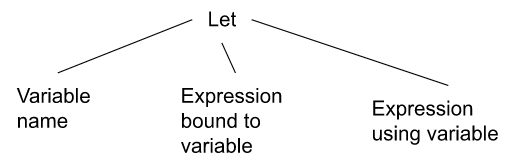
\includegraphics[width=1\linewidth]{img/ast.png}}
    \caption{AST}
    \label{fig:ast}
\end{figure}

\hspace{16}Our GNN will learn to assign a vector to each node in this tree that captures information about the functionality of that node. In the case of a “Let” expression, the functionality that we wish to use to describe the variable is the root of the “Expression bound to variable” subtree. A well-trained network will store information in the root of a tree summarizing the logic of its descendents. We may therefore think of this node’s vector as a neural description of the logic bound to the variable.

\subsubsection{Semantically sensitive selection of actions}
\hspace{16}Actions that do not change over the course of training may be bound to a fixed index in the action space of the agent. Because the semantics do not change, the agent learns to associate the index with these fixed semantics. Variables pose a challenge because their semantics change from variable to variable (and there are infinite distinct expressions to which variables can be bound). Consequently, the “insert variable” action should not be represented to the agent as an index but as a rich vector that captures information about the logic that the variable represents. We have already proposed one such vector.

\hspace{16}In order to support the selection of this vector, we propose a new method for parameterizing the action distribution similar to the \textit{Query-Key-Value} mechanism described in \href{https://arxiv.org/abs/1706.03762}{Attention is All You Need}. At the start of training we initialize an $N \times D$ matrix $K_{fixed}$, where $N$ is the number of $fixed$ actions with consistent semantics and $D$ is the hidden-size of our GNN. During training, we augment $K_{fixed}$ with a matrix, $K_{var}$, which stacks the variables corresponding to in-scope variables (using the vector representation described in the previous section). Let $k$ be the full matrix, containing both $K_{fixed}$ and $K_{var}$. $k$ has dimensions $(N + N^t_{var}) \times D$ where $N^t_{var}$ is the number of in-scope variables, which may vary by timestep. We then select an action in two steps:
\begin{enumerate}
    \item Our actor network produces parameters for a multivariate gaussian distribution, $G(x_t)$ (where $x$ is the observation). We sample a $D$-dimensional vector $q_t$ from this distribution.
    \item We sample the action from the expression:
\end{enumerate}
\begin{equation}
    a_t \sim \textrm{softmax}(\frac{q_t^Tk}{\sqrt{D}})
\end{equation}

The probability that $a_t = a'$ is therefore:
\begin{equation}
    \textrm{softmax}(\frac{q_t^Tk_{a'}}{\sqrt{D}})
\end{equation}

where $k_{a'}$ is the $a'^{\textrm{th}}$ row of $k$. If the agent wishes to select a variable with neural description vector $k_v$, the agent need only produce a query vector $q_t$ that closely resembles $k_v$ (such that $q_t^Tk$ is large). Similarly, because $K_{fixed}$ only changes gradually (due to gradient updates) over the course of training, the agent can learn to associate rows of that matrix with fixed action semantics.

\subsubsection{Learning idiomatic variable names}
\hspace{16}Though we consider this work outside the scope of this project we suggest that the learning of idiomatic variable names should be thought of as a separate learning problem with approaches that are complementary to the methods proposed in the preceding paragraphs. One straightforward approach to this problem is to frame it as a supervised learning problem in which a network is trained to map some representation of the variable (one possible representation was discussed in the section on \hyperref[sec:neural-representation]{Neural representation of variables}) to the name actually given to that variable in a large corpus of human-written code. These names could then be substituted into the code generated by our RL-based method.








\end{document}
